\documentclass[11pt]{article}

% ------------------------------
% Packages
% ------------------------------
\usepackage[margin=1in]{geometry}
\usepackage{amsmath, amssymb, amsthm}
\usepackage{enumitem}
\usepackage{float}
\usepackage{graphicx}
\usepackage{cite}
\usepackage{hyperref}
\usepackage{fancyhdr}
\usepackage{tikz}
\usepackage{lastpage}
\usepackage{xcolor}
\usepackage{array}
\usepackage{multirow}
\usepackage{tabularx}
\usepackage{booktabs}
\usepackage{caption}
\usepackage{minted}
\usepackage{algorithm}
\usepackage{algpseudocode}
\newcolumntype{Y}{>{\raggedright\arraybackslash}X}

% ------------------------------
% Global Settings
% ------------------------------
\setlength{\parindent}{0pt}
\setlength{\parskip}{6pt}
\setlength{\headheight}{14pt}
\hypersetup{
  colorlinks=true,
  linkcolor=blue,
  citecolor=black,
  urlcolor=blue
}
\usetikzlibrary{arrows.meta,positioning}
\usetikzlibrary{shapes.geometric}
\usemintedstyle{friendly}

% ------------------------------
% Metadata
% ------------------------------
\newcommand{\studentName}{Faaiz Khan}
\newcommand{\studentRollNo}{25280051}
\newcommand{\courseCode}{AI600}
\newcommand{\courseName}{Deep Learning}
\newcommand{\hwNumber}{Assignment \#2}
\newcommand{\professorName}{Prof. Dr. Momin Uppal}
\newcommand{\taNames}{Muhammad Aleem Shakeel, Muhammad Usman, Muhammad Qasim Ayub, Usman Ahad}
\newcommand{\dueDate}{Monday March 2, 2026}
\newcommand{\honorPledge}{%
I affirm that I have abided by the academic integrity policy. I have neither given nor received unauthorized aid on this assignment.\\
}

% ------------------------------
% Header & Footer (applies to pages AFTER the cover)
% ------------------------------
\pagestyle{fancy}
\fancyhf{}
\fancyhead[L]{\studentName}
\fancyhead[C]{\courseName}
\fancyhead[R]{\hwNumber}
\fancyfoot[C]{Page \thepage\ of \pageref*{LastPage}}

% ------------------------------
% Problem Environments
% ------------------------------
\newcounter{problem}
\newcounter{task}
\newcounter{question}

% Base "problem" environment: prints bold "Problem n." (optional short title)
\newenvironment{problem}[1][]{
  \refstepcounter{problem}%
  \par\bigskip
  \noindent\textbf{Problem \theproblem.\if\relax\detokenize{#1}\relax\else\ #1\fi}\par
  \medskip
}{\par\bigskip}

\newenvironment{task}[1][]{
  \refstepcounter{task}%
  \par\bigskip
  \noindent{\Large\textbf{Task \thetask.\if\relax\detokenize{#1}\relax\else\ #1\fi}}\par
  \medskip
}{\par}

% Variant that forces a page break at the end:
\newenvironment{problembreak}[1][]{
  \refstepcounter{problem}%
  \par\bigskip
  \noindent\textbf{Problem \theproblem.\if\relax\detokenize{#1}\relax\else\ #1\fi}\par
  \medskip
}{\par\bigskip\clearpage}

\newenvironment{question}[1][]{
  \refstepcounter{question}%
  \par\bigskip
  \noindent{\Large\textbf{Question \thequestion:\if\relax\detokenize{#1}\relax\else\ #1\fi}}\par
  \medskip
}{\par\bigskip}

% ------------------------------
% Document
% ------------------------------
\begin{document}

% -------- Cover Page (no header/footer) --------
\begin{titlepage}
  \thispagestyle{empty}
  \centering
  \vspace*{2cm}
  {\Large \courseCode\ \courseName\par}
  \vspace{0.5cm}
  {\LARGE \hwNumber\par}
  \vspace{0.5cm}
  {\large Due: \dueDate\par}
  \vfill

  \newcolumntype{L}[1]{>{\raggedleft\arraybackslash}m{#1}}
  \newcolumntype{C}[1]{>{\centering\arraybackslash}m{#1}}

  \begin{tabular}{@{} L{0.22\textwidth} C{0.68\textwidth} @{}}
    \textbf{Professor:} & \professorName \\
    \textbf{TA(s):}     & \taNames \\
    \textbf{Student:}   & \studentName \\
    \textbf{Roll No.:}  & \studentRollNo
  \end{tabular}
  
  \vfill

  \begin{minipage}{0.9\textwidth}
    \small
    \textbf{Honor Pledge:}\\[2pt]
    \honorPledge
    \noindent All work, code implementation, and data for this assignment can be found at the following public GitHub repository: \\
\url{https://github.com/FaaizKhan1999/ai600-assignments/tree/main/assignment-02}
    \vspace{1.2cm}
  \end{minipage}
\end{titlepage}

% Start page numbering from 1 after the cover
\setcounter{page}{1}

\begin{question}[The "Quick, Draw!" Challenge]
  {\large\textbf{Part A: The Pancake (Width Focus)}}\\
  In this part, a shallow but wide network was trained. This \texttt{pancake\_model} has 2 hidden layers, with 1024 and 2048 neurons per layer respectively.\\
  The two plots below provide the training and validation accuracy per epoch, as well as the average loss per epoch for this model.
  \begin{figure}[H]
    \centering
    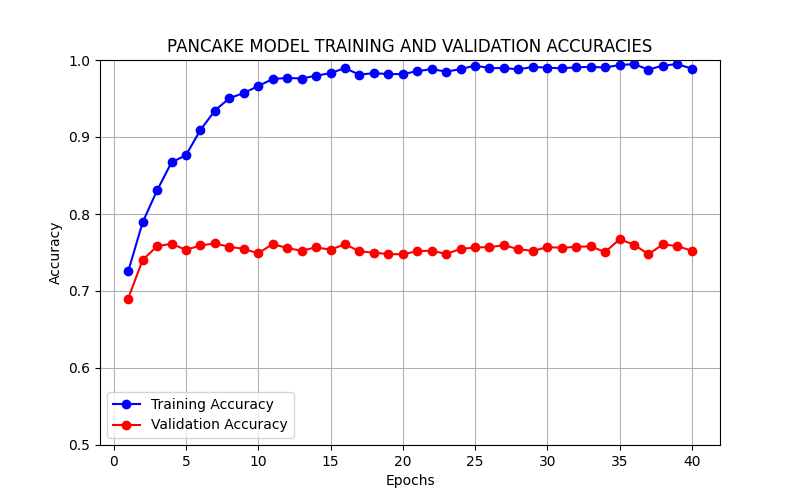
\includegraphics[scale=0.5]{figs/pancake_accs.png}
    \caption{The per epoch training and validation accuracies for the pancake model.}
  \end{figure}
  \begin{figure}[H]
    \centering
    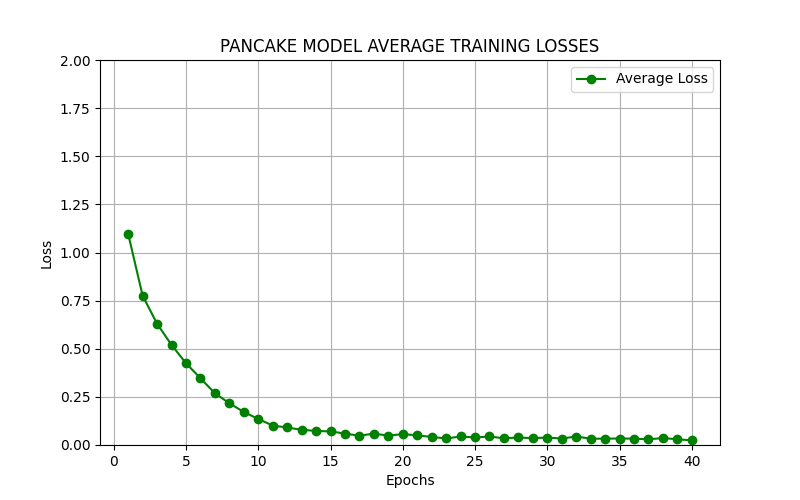
\includegraphics[scale=0.5]{figs/pancake_loss.png}
    \caption{The per epoch average loss for the pancake model.}
  \end{figure}
  From the images above, it can be seen that the model's training accuracy becomes almost perfect (around 99\%) as it goes through its training cycles whereas its validation accuracy plateaus very early at approximately 74\%. This plateau can be seen as early as epoch 5. Therfore, it can be inferred that the model stops generalising at around that time and any learning beyond that is just overfitting. This is also reinforced by the loss curve which show that there is very minimal learning happening beyond epoch 10.\\[1em]
  {\large\textbf{Part B: The Tower Model (Depth Focus)}}\\
  In this part, a deep but narrow network was trained. This \texttt{tower\_model} has 5 hidden layers with 128, 256, 512, 256, and 128 neurons per layer respectively.
  The two plots below provide the training and validation accuracy per epoch, as well as the average loss per epoch for this model.
  \begin{figure}[H]
    \centering
    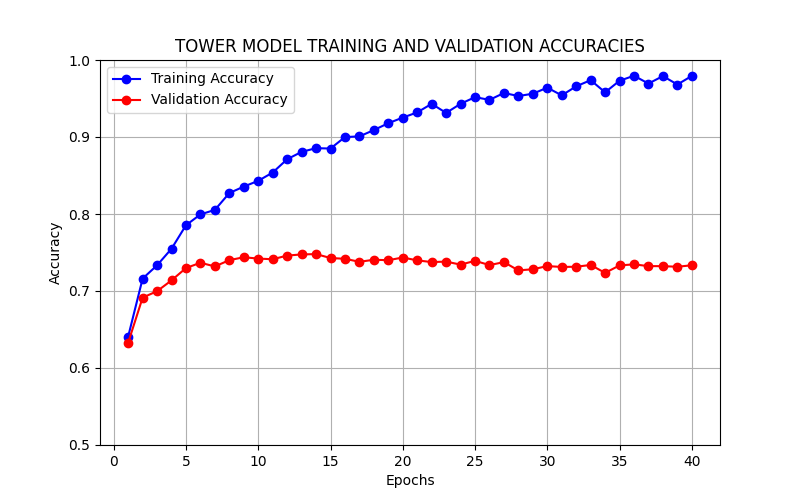
\includegraphics[scale=0.5]{figs/tower_accs_no_bn.png}
    \caption{The per epoch training and validation accuracies for the tower model.}
  \end{figure}
  \begin{figure}[H]
    \centering
    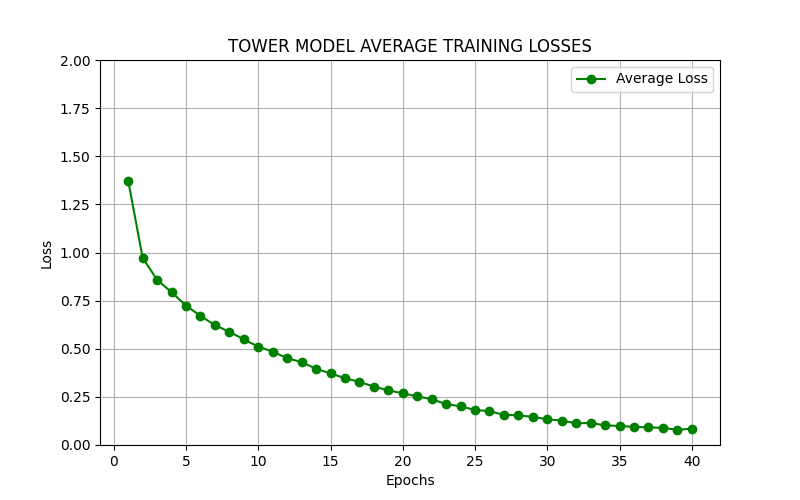
\includegraphics[scale=0.5]{figs/tower_loss_no_bn.png}
    \caption{The per epoch average loss for the tower model.}
  \end{figure}
  From the images above, it can be seen that the model's training accuracy steadily increases until it reaches a very high number (around 97\%) whereas --- akin to the pancake model --- its training accuracy plateaus at around 73\%. This plateau can be seen as early as epoch 5. Once again, the inference dictates that the model stops generalising and starts overfitting. The loss curve also has a much steadier decrease compared to the pancake model.\\
  As the network gets deeper, it may run into training difficulties in the form of vanishing gradients. While the inference from the plots cannot reliably assert that this is actually the case, the network was retrained using 1D Batch Normalisation to see if that resulted in an improvement in the network. The related plots are provided below.
  \begin{figure}[H]
    \centering
    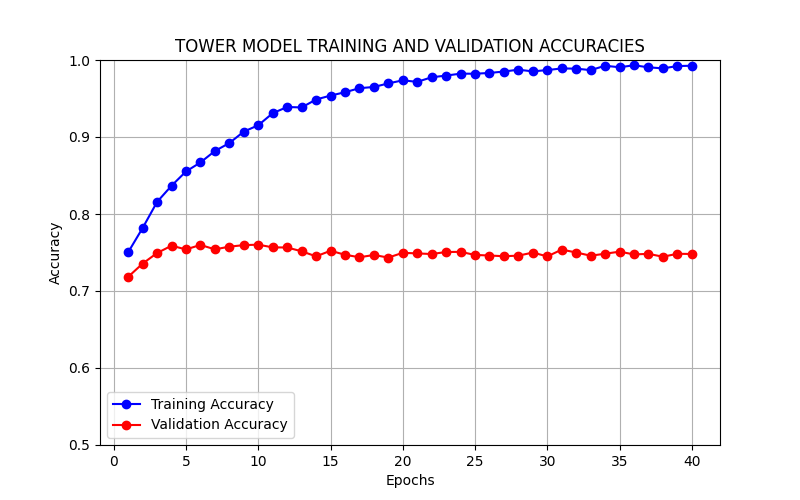
\includegraphics[scale=0.5]{figs/tower_accs.png}
    \caption{The per epoch training and validation accuracies for the tower model with Batch Normalisation.}
  \end{figure}
  \begin{figure}[H]
    \centering
    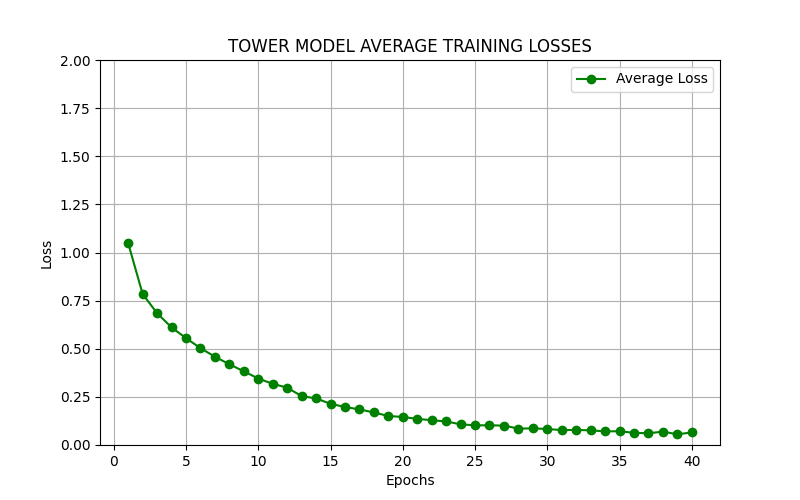
\includegraphics[scale=0.5]{figs/tower_loss.png}
    \caption{The per epoch average loss for the tower model with Batch Normalisation.}
  \end{figure}
  As can be seen in the plots, there is a noticeable difference in the training and validation accuracies of the network after Batch Normalisation is worked into the model. The training accuracy now steadily increases to nearly perfect (around 99\%) as with the pancake model and the network even outperforms the pancake model, albeit marginally with a validation accuracy that plateaus at 75\% but peaks at 76\% at around 5 epochs. This is also the first time the effect of overfitting and the loss of generalisation is actually noticeable. As the epochs increase, the training accuracy increases but the validation accuracy starts decreasing.

  \pagebreak

  {\large\textbf{Part C: The Champion (Leaderboard Submission)}}\\
  To summarize the information from the first two parts, a table with the performances of each network trained over 10 epochs is provided below.
  \begin{table}[H]
    \centering 
    \begin{tabular}{@{}lccc@{}}
        \toprule
        \textbf{Model} & \textbf{Training Accuracy (\%)} & \textbf{Validation Accuracy (\%)} \\ \midrule
        Pancake Model                     & 96.86\%  & 76.18\% \\
        Tower Model                       & 84.28\%  & 74.73\% \\
        Tower Model (Batch Normalization) & 92.21\%  & 76.36\% \\
        \bottomrule
    \end{tabular}
    \caption{Performance Comparison of Network Architectures}
  \end{table}
  The final model is an MLP with 4 hidden layers. The layers and their components are provided below.
  \begin{itemize}
    \item \textbf{Input Layer:} 784 units.
    \item \textbf{Hidden Layer 1:} 512 neurons, BatchNorm, GELU activation, Dropout (0.3).
    \item \textbf{Hidden Layer 2:} 256 neurons, BatchNorm, GELU activation, Dropout (0.2).
    \item \textbf{Hidden Layer 3:} 128 neurons, BatchNorm, GELU activation, Dropout (0.1).
    \item \textbf{Output Layer:} 15 units.
  \end{itemize}
  Moving on, the different training hyperparameters/features used are also given below:
  \begin{itemize}
    \item \textbf{Label Smoothing:} Cross-entropy loss with a rate of $0.1$. 
    \item \textbf{Optimizer:} Adam with a Learning Rate of $0.002$.
    \item \textbf{Regularization:} L1 regularization ($\lambda=8\times10^{-5}$).
    \item \textbf{Learning Rate Scheduler:} \texttt{OneCycleLR}.
    \item \textbf{Activation Function:} GELU.
  \end{itemize}
  The model demonstrated gradual convergence over the 40 epochs.
  \begin{table}[H]
  \centering
  \begin{tabular}{lc}
    \toprule
    \textbf{Metric} & \textbf{Score} \\ \midrule
    Training Accuracy & 94.17\% \\
    Validation Accuracy & 82.73\% \\
    \textbf{Test Accuracy} & \textbf{82.06\%} \\ \bottomrule
  \end{tabular}
  \caption{Final Performance Metrics}
  \end{table}
  \begin{figure}[H]
    \centering
    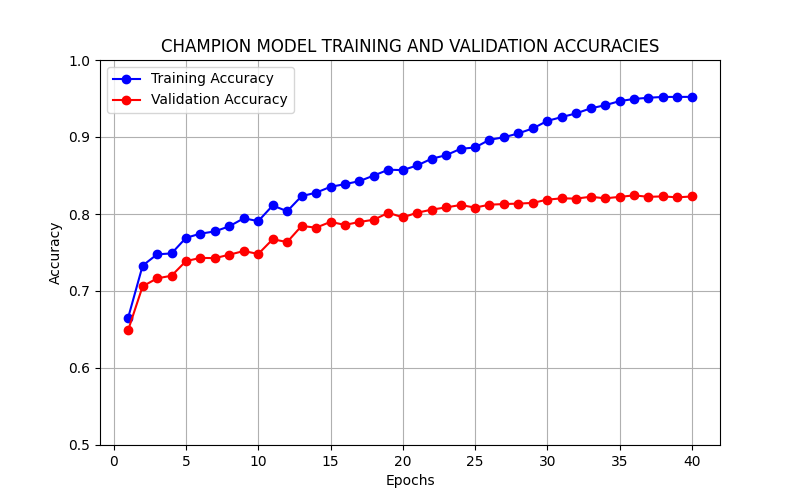
\includegraphics[scale=0.5]{figs/champion_accs.png} 
    \caption{The per epoch training and validation accuracies for the champion model.}
  \end{figure}
  Finally, the network was trained over 37 epochs and contains only $569,871$ parameters, well below both thresholds.

  {\large\textbf{Part D: Theoretical Analysis}}\\
  1. The pancake model trained had $2,933,775$ parameters whereas the tower model had only $433,807$. Even though the difference in the performance of these models was barely noticeable (after the addition of Batch Normalisation to the tower model), there is some intuition behind preferring a deeper architecture despite what the Universal Approximation Theorem may state. Firstly, the theorem states that a single hidden layer is sufficient to approximate any continuous function. However, it does not state that the resulting model will be practical. The important thing to note here is that approximation is not the end goal, the trainability and usefulness of the model is. Secondly, images are inherently heirarchical, meaning that they are created of different components which are comprised of some basic shapes which are made up of lines and so on. Think of each layer as an abstraction that may recognise these patterns hidden inside images.\\
  2. The confusion matrix generated by the champion model's predictions on the validation set is provided below. The main takeaway from this matrix is perhaps unsurprising. The network struggles most with differentiating between shapes that look similar or have similar features: pizza/wheel, basketball/football, clock/compass; in descending order of confusion. For almost all of these pairs, this can be chalked up to aleatoric uncertainty. In a grayscale $28\times28$, a pizza with 8 slices and a wheel with rims (as an example) would almost be indiscernable. This same logic could be applied to a basketball and a football (sperical objects), or a clock and a compass (circular with arms/needles).
  \begin{figure}[H]
    \centering
    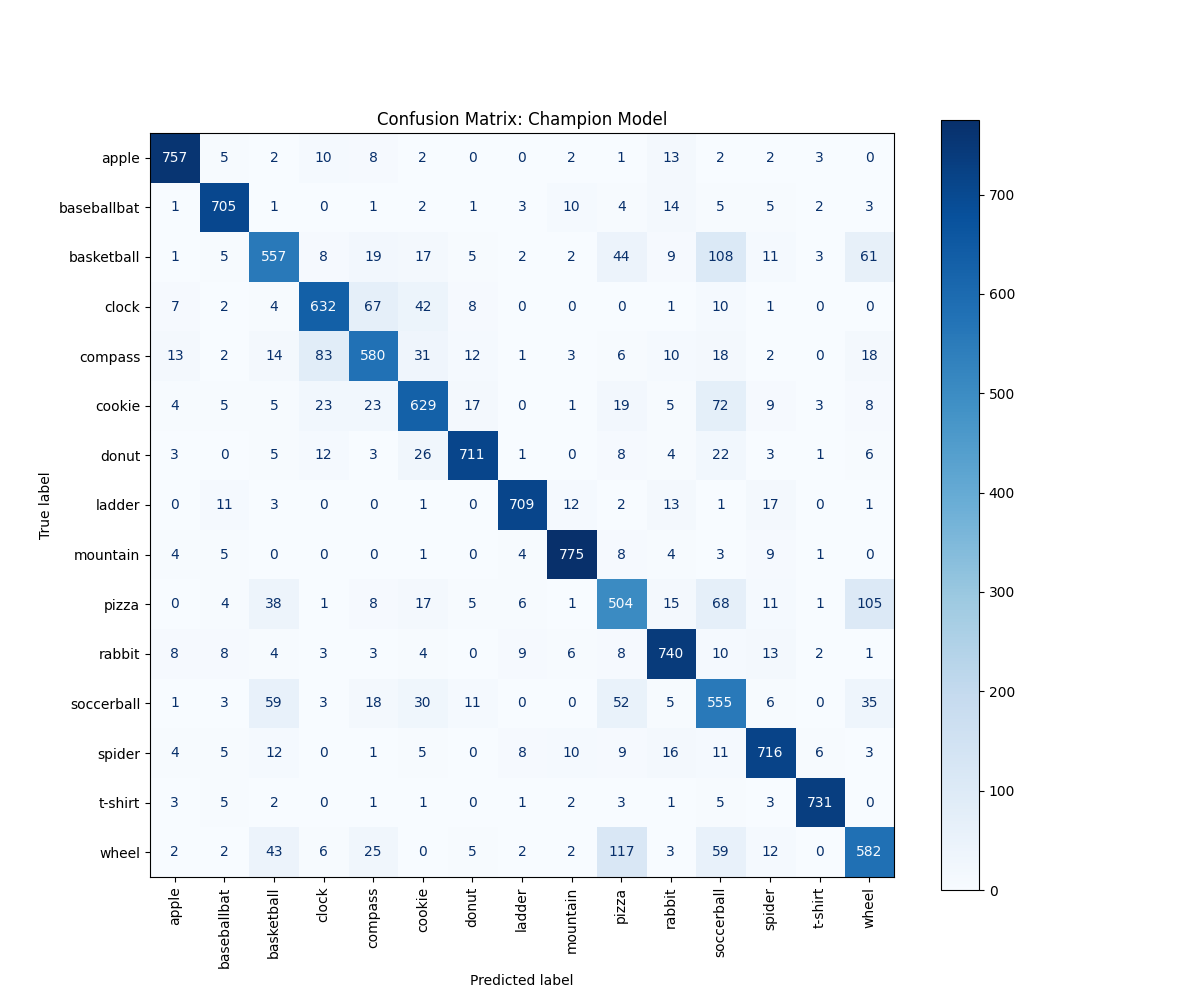
\includegraphics[scale=0.5]{figs/conf-matrix.png} 
    \caption{The champion models' confusion matrix evaluated on the validation set.}
  \end{figure}

  {\large\textbf{Part E: Report and Rationale}}
  When it comes to how the depth and width were chosen, the answer is simply a lot of trial and error. I initially noticed that both the pancake and the tower model exhibited huge amounts of overfitting, so Itried to look for a happy medium before settling for the architecture mentioned in Part C. The overfitting has by no means been eradicated but its effects have been mitigated by some margin.\\
  The overfitting was combatted by making a lot of small changes to the network: these involve label smoothing, early stopping, dropout, learning rate scheduling.\\
  The table below compares the three models and how well they performed.
  \begin{table}[H]
    \centering 
    \begin{tabular}{@{}lcccc@{}}
        \toprule
        \textbf{Model} & \textbf{Parameters} & \textbf{Training Epochs} & \textbf{Training Acc.} & \textbf{Validation Acc.} \\ \midrule
        Pancake Model   & $2,933,775$ & 40 & 96.86 & 76.18 \\
        Tower Model     & $433,807$ & 40 & 92.21 & 76.36 \\
        Champion Model  & $569,871$ & 37 & 94.17 & 82.73 \\
        \bottomrule
    \end{tabular}
    \caption{Performance Comparison of Network Architectures Including the Champion Model.}
  \end{table}
\end{question}

\pagebreak

{\Large\textbf{GEN AI USAGE}}\\[1em]
All the content written in the report is written explicitly by me. Gen AI tools were only ever used as an aid for conceptual understanding and had no direct role in solving the questions. All research related to decision-making an understanding was also done by me.\\
The relevant content pertaining to the assignment was also written by myself. VS Code's Copilot was used to help provide boilerplate code instead of writing any of the logic.

\end{document}
